\documentclass{sigchi}

% Use this command to override the default ACM copyright statement (e.g. for preprints). 
% Consult the conference website for the camera-ready copyright statement.
\toappear{
Permission to make digital or hard copies of all or part of this work for personal or classroom use is granted without 	fee provided that copies are not made or distributed for profit or commercial advantage and that copies bear this notice and the full citation on the first page. Copyrights for components of this work owned by others than ACM or the author must behonored. To copy otherwise, or republish, to post on servers or to redistribute to lists, requires prior specific permission and/or a fee. \\
{\confname{UbiComp '13}}, Sept 9-12, 2013, Zurich, Switzerland.\\
Copyright 2013 ACM 978-1-4503-1770-2/13/09...\$15.00.
}

% Arabic page numbers for submission. 
% Remove this line to eliminate page numbers for the camera ready copy
%\pagenumbering{arabic}


% Load basic packages
\usepackage{balance}  % to better equalize the last page
\usepackage{graphics} % for EPS, load graphicx instead
\usepackage{times}    % comment if you want LaTeX's default font
\usepackage{url}      % llt: nicely formatted URLs

% llt: Define a global style for URLs, rather that the default one
\makeatletter
\def\url@leostyle{%
  \@ifundefined{selectfont}{\def\UrlFont{\sf}}{\def\UrlFont{\small\bf\ttfamily}}}
\makeatother
\urlstyle{leo}


% To make various LaTeX processors do the right thing with page size.
\def\pprw{8.5in}
\def\pprh{11in}
\special{papersize=\pprw,\pprh}
\setlength{\paperwidth}{\pprw}
\setlength{\paperheight}{\pprh}
\setlength{\pdfpagewidth}{\pprw}
\setlength{\pdfpageheight}{\pprh}

% Make sure hyperref comes last of your loaded packages, 
% to give it a fighting chance of not being over-written, 
% since its job is to redefine many LaTeX commands.
\usepackage[pdftex]{hyperref}
\hypersetup{
pdftitle={SIGCHI Conference Proceedings Format},
pdfauthor={LaTeX},
pdfkeywords={SIGCHI, proceedings, archival format},
bookmarksnumbered,
pdfstartview={FitH},
colorlinks,
citecolor=black,
filecolor=black,
linkcolor=black,
urlcolor=black,
breaklinks=true,
}

% create a shortcut to typeset table headings
\newcommand\tabhead[1]{\small\textbf{#1}}


% End of preamble. Here it comes the document.
\begin{document}

\title{Rhapsodize: Mobile Application for Improving Public Speaking Skills Through Training of Speech Disfluencies}

\numberofauthors{2}
\author{
  \alignauthor Charles Tark\\
    \affaddr{Cornell University}\\
    \affaddr{516 University Ave, Ithaca, NY 14850}\\
    \email{cyt25@cornell.edu}\\
  \alignauthor Mark Yoon\\
    \affaddr{Cornell University}\\
    \affaddr{311 Eddy St., Ithaca, NY 14850}\\
    \email{yhy5@cornell.edu}\\
}

\maketitle

\begin{abstract}
Speech disfluencies are a common part of human conversation. From public speeches to everyday conversation, words such as “like,” “um,” and “you know” permeate our vocabulary. A paper in the Journal of Psycholinguistic Research looks for a relationship between disfluency and speech comprehension. It concludes that speech “disfluency affects core language comprehension processes” [2]. Additional studies have been done to identify why we say these words in our speech. A study published in the Language and Linguistics Compass Journal concludes that “there is little evidence to suggest that they are intentionally produced, or should be considered to be words in the conventional sense” [1], indicating that these words are purely hesitation disfluencies. Now that we have established these speech disfluencies are detrimental to communication and speech giving, we set out to create a tool to help individuals get rid of this habit. Our application, Rhapsodize, takes user speech as an input and notifies the user when/how often these words are said. The user is able to view their relative performance over time regarding their speech patterns, tracking their improvement in avoiding these crutch words.
\end{abstract}

\keywords{
	speech disfluencies; natural language processing; crutch word detection; speech recognition; mobile computing
}

\category{H.1.2}{User/Machine Systems}{I.2.7.}{ Natural Language Processing}

\terms{
	Human Factors; Design; Experimentation
}

\section{Introduction}

Public speaking is a very common fear. Speech ranges across a lot of different scenarios -- after all, it is the main method by which we communicate with each other. Whether it is giving a speech or talking amongst friends, it is very common for people to have slight speech impediments. Phrases such as ``like'' and ``um'' permeate our speech and oftentimes the speaker does so unknowingly. After becoming so comfortable using these “crutch” words, it’s very hard for an individual to restrain his or herself from doing so.

Our application, Rhapsodize, aims to prevent this problem. We hypothesize that notifying a user of crutch word usage in real time will have a beneficial outcome in reducing the frequency of crutch word usage. When saying a crutch word in conversation or while practicing a speech, Rhapsodize will notify the user that a crutch word has been said, hopefully guiding the user to less and less frequent usage of these words. Over time, the user will be behaviorally conditioned to avoid saying these words, either consciously or subconsciously, thereby improving their overall speech giving performance.

Rhapsodize is an Android application that uses Carnegie Mellon University`s CMU Sphinx speech recognition API [7] to continuously detect speech for crutch word occurrences. It notifies the user when these words are said and also keeps track of how often they are said so that the user can log progress. Though ideally the application would be used throughout the day to keep track of the user’s speech in daily conversation, this would lead to privacy concerns as well as many more technical challenges in making the application more than simply a proof of concept. As a result, Rhapsodize is to be used as a more situational, speech-giving improvement tool. The user places the phone running Rhapsodize in front of him or herself (or inside his or her pocket through the use of an external microphone) while practicing giving a speech and the device will detect and count crutch word occurrences. 

Our experimental design seeks to determine to what extent such a tool would benefit users in improving their speech giving skills. Ideally, the use of the application would allow users to become more fluent in their speaking by allowing them to train themselves over time to speak with minimal inclusion of such speech disfluencies. Long term, we hope to distribute a fully-realized version of our application with additional features, including captured transcriptions and data visualizations for general and widespread public use.


\section{Related Work}

There has been a lot of interest in interfaces to help people with public speaking. Researchers have been developing several different systems in this domain. 

M. Iftekhar Tanveer et al. discuss their application, Rhema, in their paper, \textit{Rhema: A Real-Time In-Situ Intelligent Interface to Help People with Public Speaking} [4]. Their system involves a user wearing Google Glass and receiving regular feedback regarding their speech. The system aims to provide live feedback when giving a speech. The system keeps track of speech speed and volume. If either one is above or below the ideal value, the user is notified via the Google Glass display. Their quantitative and qualitative analysis concluded that their system helped users in giving a higher quality speech.

Mohammed Hoque et al. made a system of their own that instead of providing live feedback during an actual speech, is a coach that helps train users to have better conversational skills. This is discussed at length in their paper, \textit{MACH: My Automated Conversation coacH} [3]. Their results indicate that students who interacted with MACH had overall improved interview scores as opposed to the control group of students. 

These are some of the many approaches to speech analysis and feedback systems that exist today. Speech is a very complex and broad topic and an application that encorporates all aspects of speech would include a lot of different features. Although both of the aforementoned systems attempt to solve a similar problem as Rhapsodize, they don't tackle exactly the same problem. Detecting crutch words is another way to improve speech mechanics and improve conversational and public speaking skills.

\subsection{Application Description}

Rhapsodize is intended to be a tool that a user can access on the go. The three components that are necessary for Rhapsodize to function as intended are a microphone, user-facing screen, and processor. Given these prerequisites, it made the most sense to make a mobile application. Our application is built on the Java-based Android mobile application platform (4.1+) [5]. The design decisions we made when creating the application hinged upon the use case that we wanted to have. As a result, the user-interface of the application reflects how we wanted the application to be used. Past the user-interface, the implementation of natural language processing to perform speech recognition is crucial to the functionality of the application. As a result, a lot of effort was put into making the recognition as accurate as possible.

\subsection{User Interface}

When designing our application, we had two use cases in mind. The first was to have the application constantly open in the user’s background. A mic, via a bluetooth headset, would capture the user’s speech throughout the day, counting the times various crutch words were said in everyday conversation. This data can then show overall speech patterns of the user. The second use case was to have the application used as a utility to help users practice their speech in a controlled, quiet setting - i.e. the user would use the application to explicitly improve their speech. 

There are some concerns with the first use case. Firstly, there would undoubtedly be some privacy concerns. In order to capture speech, the user’s mic would have to be constantly on in the background. Not only would the mic capture all of the user’s own speech, it would also capture the speech of all of those within earshot of the user. Secondly, having the mic capture the user’s speech amidst everyday ambient noise makes speech recognition through natural language processing extremely more difficult. When we initially created and tested our application for this use case, there were enough false positives that the data integrity was compromised and no information of any significance would be obtained by the user.

Given both the ethical and technical concerns surrounding the first use case, we modified the application to fit the second model instead. The user opens the application whenever they want to practice their speech. Once the application is open, the user can press a button to start the recognition. For best performance, a bluetooth mic or inline headphone mic should be used while the phone is placed in the user’s pocket. If such a mic is not available, the phone should be placed on a surface in front of the user, with the mic on the phone unobstructed. Once the recognizer is started, the application starts keeping track of the frequency of crutch words said and when. 

Another important consideration we had when designing the application was how to notify the user of crutch word usage. Because the application is mobile-based, notifications can be made through a vibration or audio alert. A more important question is whether or not notifications are beneficial. Constantly notifying the user of a notification could have negative effects on the user as it may lead to nervousness. Since everybody is unique in how they respond to feedback, Rhapsodize is designed such that the user can decide what kind of notification is received upon crutch word occurrence. The options we have are no notifications, vibration only, ring only, or both vibration and ring. 

Once the user is finished practicing, the user presses a button to stop the recognition. The results page shows how many times each crutch word was said and how long the practice lasted. The user can then use this information to determine overall performance for the given session. There are many things that can be done to improve the user interface but they are not currently implemented. Discussion of future improvements can be found later in this paper.

\begin{figure}[!h]
\centering
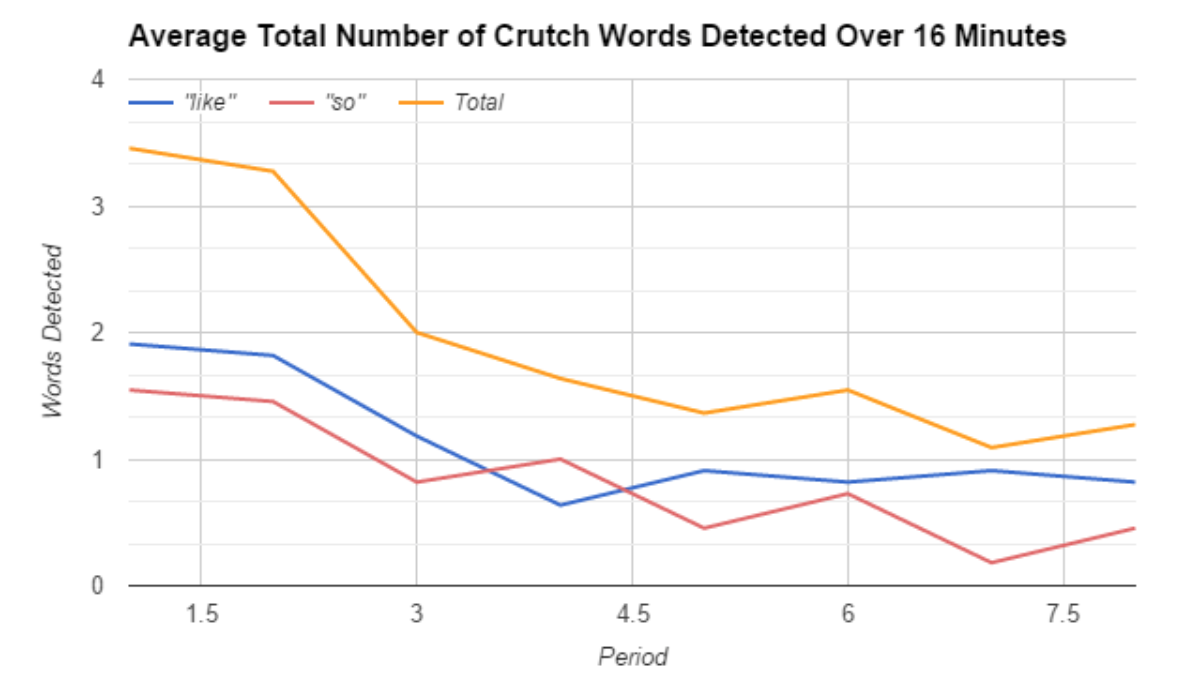
\includegraphics[width=0.9\columnwidth]{graph}
\caption{The primary modes of the application: The recordings list, the profile page, and the review/record page.
}
\label{fig:figure1}
\end{figure}


\subsection{Technical Implementation}

The usefulness of our application is entirely dependant on the accuracy of our speech recognition. As a result, a lot of emphasis is placed on this computation. There were two main application program interfaces (API’s) to consider when it comes to Android speech recognition and natural language processing. The first is the Google native speech recognition API [6]. Google’s speech recognition is top-class. However, there are several drawbacks for this particular API. In general, the service is not very flexible. The process is completely abstracted and encapsulated, which is good for most people, but because we are using our application in a very specific way to search for keywords, being able to modify the process is a desirable feature. Furthermore, the Google speech recognition API does not support offline processing capabilities which means that it’s possible that the computation could be bottlenecked by the internet speed. However, the most important limitation that this API had was the lack of continuous keyword spotting. For our application to function as we want to, notifying the user in real time of crutch word usage, the speech processing needs to be done in real time. Google’s speech recognition library does not do this. 

As a result, we used CMU Sphinx [7]	, a speech recognition API that is designed specifically for low-resource platforms (such as mobile devices). Not only does the CMU Sphinx Android port allow for continuous keyword spotting, it also allows for heavy customization in the natural language processing computation. 

A lot of fine tuning of the speech recognition was needed in order to get decent accuracy from the system. CMU Sphinx performs signal processing to match the input sound against the phonetics of the words in its dictionary. A similarity matrix is calculated by comparing the input and the dictionary; if the similarity value crosses a certain threshold, a notification goes off, saying that there has been a match. Not only can we calibrate this threshold value, we can also change the dictionary that CMU Sphinx takes as an input. There are many trained dictionaries available and we found that one of the CMU Sphinx native dictionaries gave the best results.

In performing keyword spotting, there are some nuances to consider. Oftentimes, crutch words such as “like” can be used in context correctly -- because the speech recognizer system is not smart enough to distinguish between a correct use of “like” and it being used as a crutch word, it simply notifies the user of both. There are some methods that can be used to try to minimize these occurrences. Given a large corpus, we can train a system to calculate the probability of a sequence of words. An N-gram is a set of consecutive words given a corpus. It can be seen as a window frame of words. Given a block of text, n words are viewed at a time. Using the Markov Assumption, we can estimate the likelihood of a word appearing in a sentence given the surrounding words. For example, if the user says “she is like a rose,” the system will initially hear “she is” and find the probability that the next token is “like.” If the probability is high, then the notification will not go off, as it’s likely that the word is being used properly and vice versa. This type of natural language processing is fairly computationally heavy. We implemented a similar system that would help us eliminate a small number of false positives but quickly learned that the processing power of mobile devices is not fast enough to support such complex computations. The phone processed the computation too slowly and as a result the phone was no longer giving real time feedback, which undermines the main functionality of the device. As mobile computing becomes faster, however, this is a good strategy to eliminate false positives.

\section{Methods}

In the creation and testing of our application, we planned for the development of two distinct branches of Rhapsodize. For the testing phase of development, we modified our application specifically for testing purposes. We forked our original repository to create a separate testing environment. The original version of Rhapsodize was intended primarily for testing of viability and effectiveness of conditioning-based training of crutch words. This development branch focused mostly on achieving the desired core functionality of the application in terms of distinct keyword parsing and recognition. The testing version of the application was what we used when performing all of our volunteer-based experiments. As a result, it is somewhat limited in terms of the end-functionality that we intended and can only detect certain crutch words that have been pre-programmed. In this case, ``like,'' and ``so.''

The development branch of Rhapsodize was developed with the intent to create a production-level application ready for personal, public use. It is with this version that we intend to implement a fully featured application with tools for reviewing previously recorded transcripts as well as visualizations for the captured data. On the other hand, the testing version of the application has the experiment in mind. We want to show through our experiment that notifying the user of crutch word usage in real time has a noticable impact in decreasing user crutch word frequency. In order to show this specific effect, we needed to keep all other variables constant. Things such as content of speech, length of speech, etc., all needed to be as similar as possible such that it doesn't have any bearing on our results. Furthermore, we wanted to keep hidden to the volunteer whether or not notifications were being given. In fact, we didn't even want the volunteers to know what exactly we were testing. By only telling the volunteer that we are testing a mobile application that helps speech practices, we eliminate possibilites that users are more self-concious of their speech from knowing what the application does. By randomizing periods of notifications on and off, we can remove user bias and be able to have a fiarly objective average of crutch word frequency during the notification on and notification off periods.

The testing version of the application reflects this experiment design. It is programmed to have a sixteen minute timer, where the notification status is randomized every two minutes (but it's guaranteed for there to be 4 on and 4 off periods). The front page displays the notification status, the count during each period, and total count. This testing specific application was useful in gathering data.

Through the behavioral training of users through auditory and haptic feedback, our application seeks to improve relative user performance to a significant degree. In evaluating the effectiveness of Rhapsodize in improving general speaking patterns through the removal of speech disfluencies, we developed the following experimental design. In evaluating the results obtained through testing, we noted that due to large variations in speaking patterns per individual, there was a very diverse set of results, and depending on the user, the number and spread of crutch words detected was drastically varied.

\subsection{Experimental Design}
\begin{itemize}
\item[1.] Find 10 willing volunteers. After having them sign a consent paper, give them the phone with the testing version of Rhapsodize installed, and give them instructions for the experiment. The users are not informed of the full nature of the experiment, and specifically are not notified that crutch words will be detected. This is done as to prevent any pre-experiment bias that they may receive.
\item[2.] Give the volunteer a piece of paper with a series of questions intended to invoke an extended duration of storytelling. At this point, the volunteer will give responses to these questions while the application is in use.
\item[3.] During this time, record the number of each crutch word said during every period as well as whether or not notifications were enabled.
\item[4.] Ask the participant for subjective views on if the application was helpful in practicing their speech. (i.e. Did you feel the application helped you minimize usage of crutch words? Did you enjoy the application user interface? What aspects of the application did you like/dislike?).
\item[5.] Evaluate and analyze the gathered data. 
\end{itemize}

\subsection{Data Collection}

We rely on the cooperation of several volunteers for data collection. For the testing phase, the app collects data in eight 2-minute intervals for a total of 16 minutes. Notifications are enabled for exactly 4 of these intervals in a random order. Volunteers are given a written set of questions that invoke storytelling. The users are not told the functionality of the application; they are simply told that we are testing an application that encourages good speaking practices. As the users answer the given questions, the application notifies the user of crutch-word usage in real time via a vibration only if it is during one of the four intervals in which notifications are enabled. Each of the eight periods are set up such that a response should consume approximately one period, that is, 2 minutes. The phone is to be placed in the users’ pocket and an earpiece will be used as the input microphone during the collection.

In this manner, we are able to observe the effects of the application in real-time, without directly biasing the user’s behavior. Furthermore, after the application testing has concluded, we ask participants for their subjective views on their speaking before, during, and after the testing and examine how they perceive their own performance. We can then look at the objective and subjective data to evaluate the effectiveness of our application.

We utilize the CMU Sphinx speech recognition API to detect speech and parse the spoken words. From this, we can gauge the user’s tendency to use certain words over others, and especially detect his/her usage of key crutch words. Throughout testing, the presence of these specific words will be recorded and analyzed with respect to time and application state.  For each of the randomized, two-minute long periods during which the application was being used, we recorded the number of times that the crutch words “like,” and “so,” were used. Aside from the automatically produced vibration notifications, the user was not interacted with during his or her speech. We performed a similar test for each of the other volunteers, trying as best as possible to avoid creating bias in anticipating the nature of the experiment.

From the crutch word frequency values that we obtain from the testing applications, we gain the quantitative data. From the brief questionnaire that we ask the volunteers, we get the quantitative data for the experiment. 

\begin{figure}[!h]
\centering
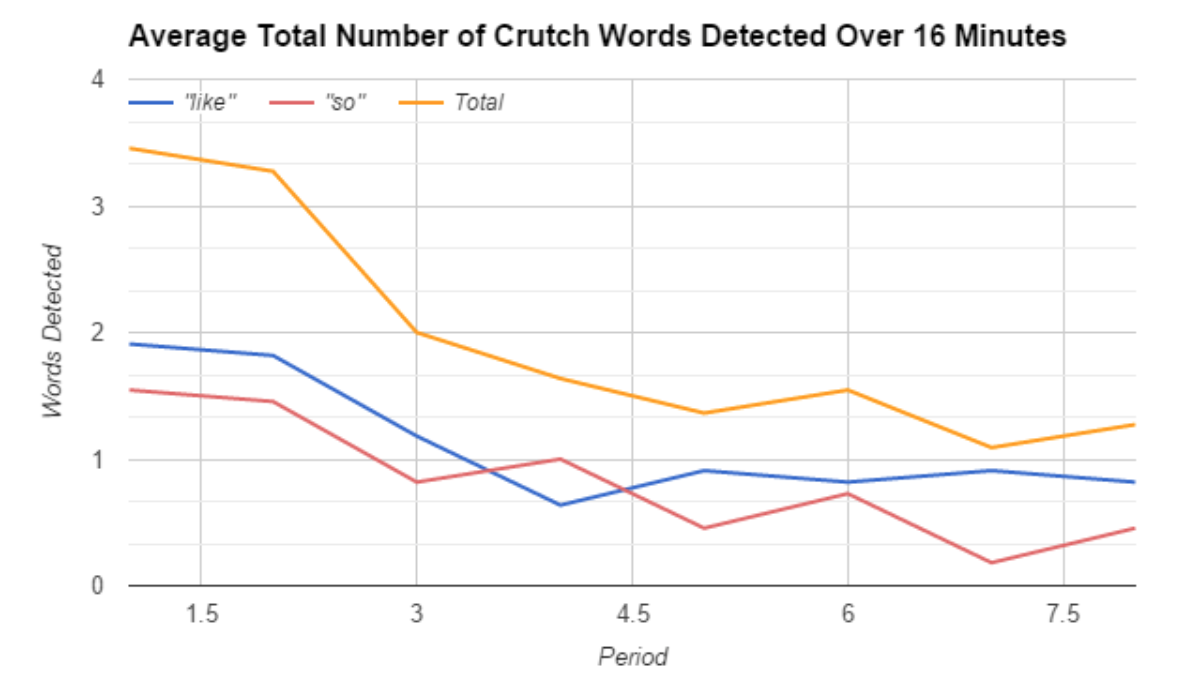
\includegraphics[width=0.9\columnwidth]{graph}
\caption{Data collected from 10 user volunteers over a duration of 16 minutes.
}
\label{fig:figure2}
\end{figure}


\begin{figure}[!h]
\centering
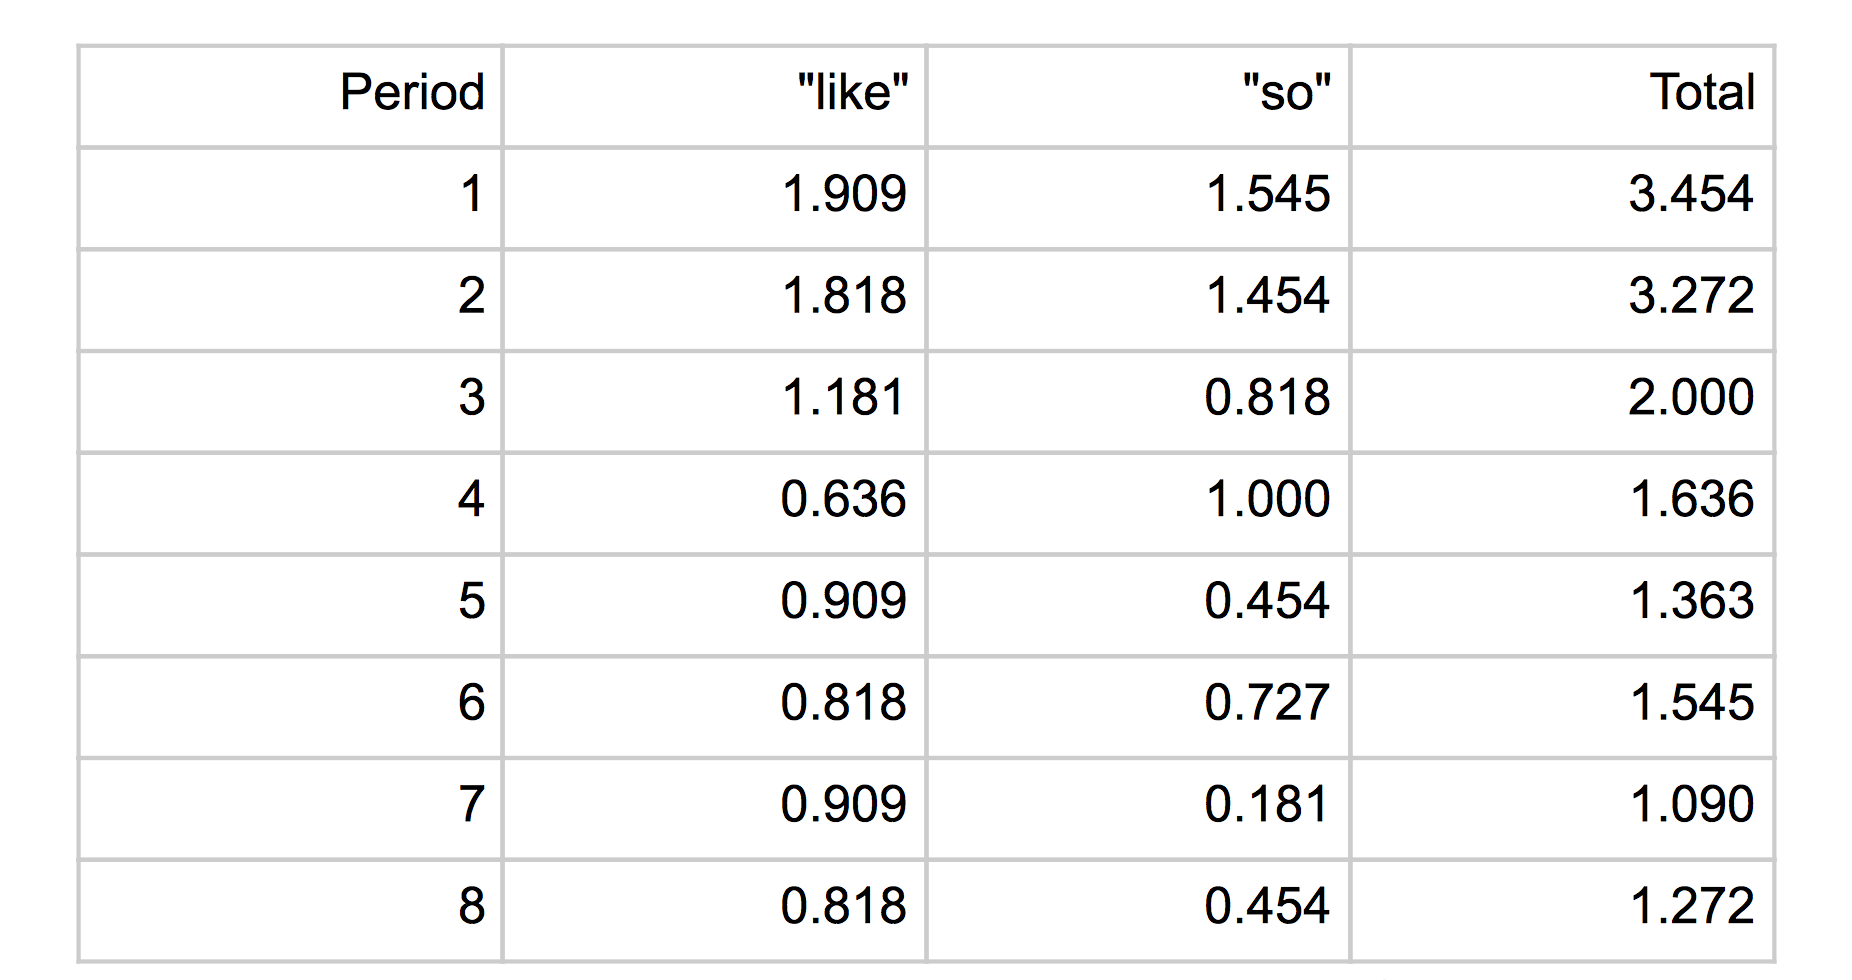
\includegraphics[width=0.9\columnwidth]{table}
\caption{Average crutch words detected for each 2 minute period over 10 volunteers
}
\label{fig:figure3}
\end{figure}


\section{RESULTS AND EVALUATION}

For the initial testing phase, we collected the number of times that the users said the words “like” and “so”, keeping track of the app’s notify/not-notify status. We randomized the notification status to  eliminate user bias when collecting data. Here are some of the observations we were able to make upon examining the data:

\begin{itemize}
\item There was a distinct correlation between when notifications were enabled and when notifications were disabled. When notifications were enabled, users said 1.12 fewer crutch words per 2 minute interval on average.
\item The spikes in our data can be attributed to the toggle-status between each interval. When notifications are enabled for two consecutive intervals, there is a very clear decrease in crutch word frequency as opposed to when notifications are toggled from on to off, where the frequency decreased less dramatically. We have hypothesized that such results are due to the nature of the notifications itself. There is a delay between when the notification state is toggled and when the user performance begins to reflect that change. As more notifications are triggered, the user responds to a greater degree, reducing the number of crutch words he or she utters.
\item There were also a few variations in the behavior of the volunteers as notification-enabled periods were interleaved in a randomized manner. For example, there were scenarios in which users would only be influenced by the notifications of the application after several periods. In these cases, the periods were arranged such that the users began speaking and continued to do so over two and sometimes three periods. Due to these few instances, there were noticeable outliers in our data.
\item Post-recording, the users noted that the vibration notification made them more aware of their speech and led to them to saying their crutch words less frequently. Furthermore, several were interested in a fully-featured, production version of the application for their own personal use.

Judging from both the difference in crutch word frequency between notifications enabled and disabled as well as the general downward trend of the graph displayed, we can draw the conclusion that notifying users via  a vibration helps decrease speech disfluencies. Furthermore, the users, almost unanimously, noted that the notification of crutch word usage helped them avoid saying them throughout the course of them talking. A couple users mentioned that the notifications made them slightly nervous and self-conscious of their speech but that it faded over the course of the 16 minute trial. Both objectively and subjectively, the data indicates that Rhapsodize is effective in reducing crutch word usage.
\end{itemize}

\section{Future Work}
There can be a lot of additional work done on the mobile application in the future. Features such as sessions and internal storage would allow users to view and references their practices in their past to find trends and keep track of progress. Furthermore, building in-app graphs from data collected would be a very nice way for users to easily see how they are doing over time. Currently, crutch words that are based on phontics, such as ``um'' and ``uh'' are very hard to detect as there are many false positives. In the future, we hope to be able to implement phontic detection just as well as the word detection we have currently.

Finally, creating a web application that could link to the application data via a user account would be very valuable to the user as the data would be more accessible and easier to view on a larger screen. With additonal computational power, the web application could also do more analysis on the speech practice.

\begin{figure}[!h]
\centering
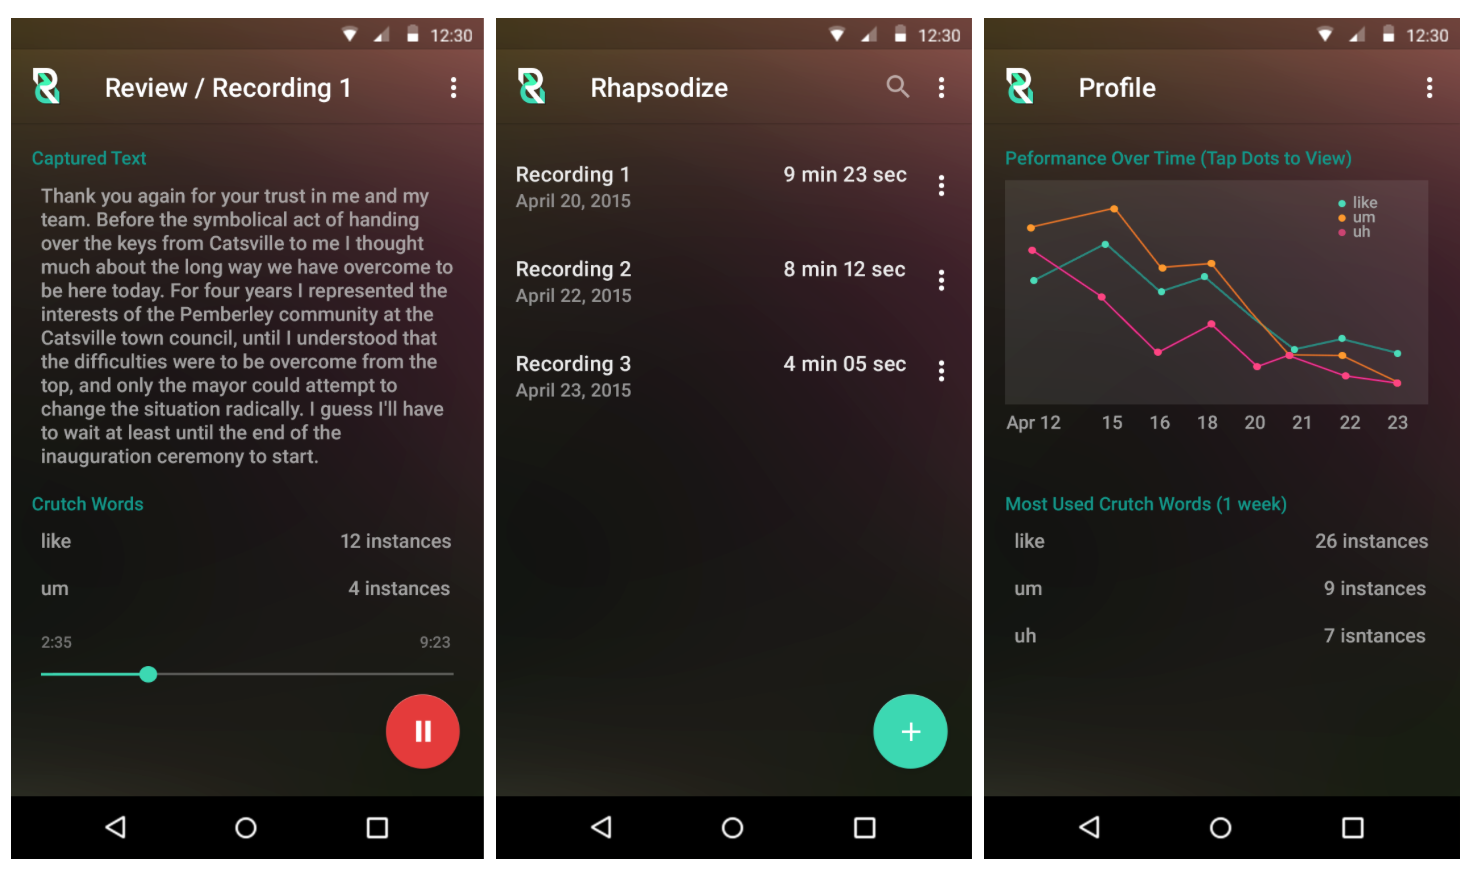
\includegraphics[width=0.9\columnwidth]{future}
\caption{User interface mock up
}
\label{fig:figure4}
\end{figure}

\section{Conclusion}

Speech analysis, processing, and training is a very broad and complex process. The field of using ubiquitous computing to make progress in the field of speech training is rapidly growing. As natural language processing becomes more advanced, it becomes easier and easier to apply it to everyone's daily lives. Mobile computing and speech libraries make way for applications such as Rhapsodize. 

From the quanlitative data we collected, even given the small sample size, there is a significant indication that the crutch word frequency declines. Not only is there a noticable difference in crutch word frequency from when notifications were on and off, there was a general downward trend in frequency over the course of the 16 minute trial. Qualitatively, users reported that the notifications were beneficial and made them more aware of their speech habits. 

Although there are many oppertunities for future work, Rhapsodize is more than a proof of concept. It is a full fledged application that, as shown by our experiment, has real merit and value as a speech tool. Not only is it free and effective, it is easy to use and can be started with a press of a button. 

\section{Acknowledgments}

We would like to thank the professors, Hane Aung and Tanzeem Choudhury for guiding the idea for our application from the experiment methodology to the technical details of the application. We would also like to thank Tauhidur Raman, the teaching assistant, for the advice and guidance on the project. We would also like to thank the volunteers for participating in our study. 

\section{References}

\begin{enumerate}
\item Corley, Martin, and Oliver W. Stewart. "Hesitation Disfluencies in Spontaneous Speech: The Meaning of Um." Language and Linguistics Compass 2.4 (2008): 589-602. Web.
\item O’Connell, Daniel C., and Sabine Kowal. "Uh and Um Revisited: Are They Interjections for Signaling Delay?" Journal of Psycholinguistic Research J Psycholinguist Res 34.6 (2005): 555-76. Web.
\item Hoque, Mohammed (Ehsan), Matthieu Courgeon, Jean-Claude Martin, Bilge Mutlu, and Rosalind W. Picard. "Mach." Proceedings of the 2013 ACM International Joint Conference on Pervasive and Ubiquitous Computing - UbiComp '13 (2013): n. pag. Web.
\item Tanveer, M. Iftekhar, Emy Lin, and Mohammed (Ehsan) Hoque. "Rhema." Proceedings of the 20th International Conference on Intelligent User Interfaces - IUI '15 (2015): n. pag. Web.
\item Google Android. Program documentation. Google Android Developers. Vers. 4.1. N.p., n.d. Web.
\item Android.speech. Android.speech. Vers. 4.1. N.p., n.d. Web.
\item CMU Sphinx. Program documentation. CMU Sphinx. N.p., n.d. Web.
\end{enumerate}

% Balancing columns in a ref list is a bit of a pain because you
% either use a hack like flushend or balance, or manually insert
% a column break.  http://www.tex.ac.uk/cgi-bin/texfaq2html?label=balance
% multicols doesn't work because we're already in two-column mode,
% and flushend isn't awesome, so I choose balance.  See this
% for more info: http://cs.brown.edu/system/software/latex/doc/balance.pdf
%
% Note that in a perfect world balance wants to be in the first
% column of the last page.
%
% If balance doesn't work for you, you can remove that and
% hard-code a column break into the bbl file right before you
% submit:
%
% http://stackoverflow.com/questions/2149854/how-to-manually-equalize-columns-
% in-an-ieee-paper-if-using-bibtex
%
% Or, just remove \balance and give up on balancing the last page.
%
\balance

% If you want to use smaller typesetting for the reference list,
% uncomment the following line:
% \small
\bibliographystyle{acm-sigchi}
\bibliography{ubicomp}
\end{document}